\chapter{CƠ SỞ LÝ THUYẾT}

\section{Các loại lỗi bảo mật phổ biến}

\subsection{Lỗ hổng kiểm soát truy cập - Broken Access Control ~\cite{chap2bib1}}
 
\paragraph{Khái niệm}

\begin{itemize}
    \item Access Control - Kiểm soát truy cập là việc kiểm soát quyền truy cập, thực hiện hành vi của người dùng trong phạm vi đã được dự định, cấp sẵn trước đó.
    \item Broken Access Control - Lỗ hổng kiểm soát truy cập là lỗ hỗng bị lợi dụng bằng những phương thức tấn công như xâm nhập, chiếm quyền sử dụng, kiểm soát các tài nguyên được bảo vệ trên hệ thống một cách trái phép. Việc này thường gây ra các hệ quả như để lộ, bị can thiệp sửa đổi thông tin một cách không mong muốn, bị phá hoại dữ liệu và thực hiện các chức năng bên ngoài phạm vi của quyền người dùng.
    \item Các CWE đáng chú ý bao gồm: CWE-200: Exposure of Sensitive Information to an Unauthorized Actor ~\cite{chap2bib4}, CWE-201: Insertion of Sensitive Information Into Sent Data ~\cite{chap2bib5}, và CWE-352: Cross-Site Request Forgery ~\cite{chap2bib6}.
\end{itemize}

\paragraph{Các lỗi thường gặp trong Broken Access Control}

\begin{itemize}
    \item Vi phạm cấu hình về đặc quyền tối thiểu. Quyền truy cập chỉ nên được cấp cho từng khả năng, nhu cầu, quyền và người dùng cụ thể thay vì cấp chung cho tất cả mọi người hoặc có những tồn tại không cần thiết.
    \begin{figure}[H]
        \centering
        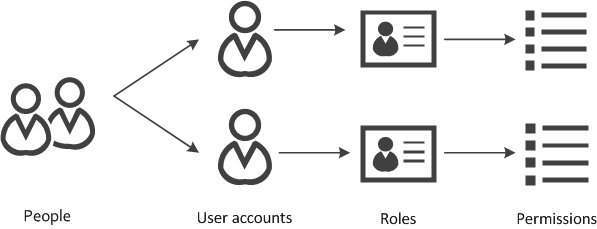
\includegraphics[width=\textwidth]{applied-thesis-chapters/chapter-2/Nguyên tắc đặc quyền tối thiểu.png}
        \caption{Nguyên tắc đặc quyền tối thiểu.png ~\cite{chap2bib2}}
    \end{figure}
    \item Có thể vượt qua phần kiểm tra quyền truy cập bằng các thao tác như mạo danh tham chiếu (Parameter Tampering) hoặc đường dẫn (Force Browsing) trong URL, thay đổi trạng thái ứng dụng và thay đổi nội dung các API gửi đi.
    \item Tham chiếu đối tượng không an toàn (Insecure Direct Object Reference - IDOR). Đối tượng có thể được tham chiếu qua nhiều phương pháp, tuy nhiên định danh duy nhất của đối tượng dùng để tham chiếu lại quá dễ đoán, không được tiền xử lý
    Như hình \ref{fib:DuLieuNhayCam} mô tả.
    \begin{figure}[H]
        \centering
        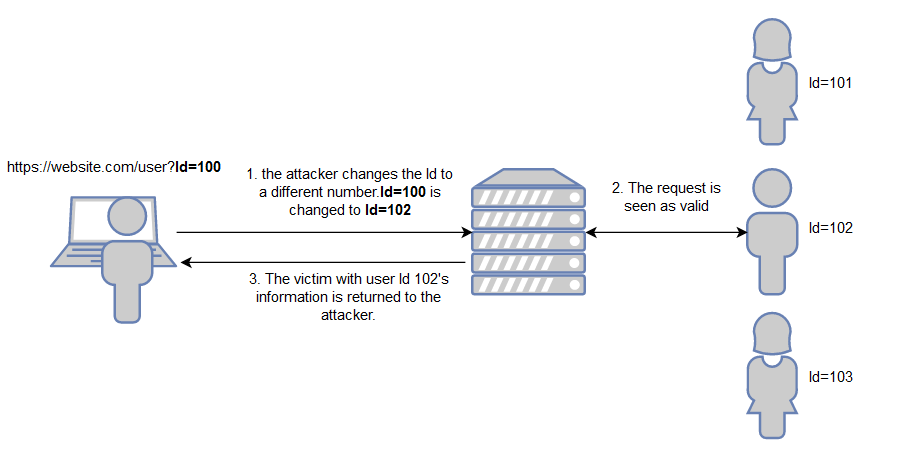
\includegraphics[width=\textwidth]{applied-thesis-chapters/chapter-2/Mô tả dữ liệu nhạy cảm có thể được tìm thấy trong URL.png}
        \caption{Mô tả dữ liệu nhạy cảm có thể được tìm thấy trong URL ~\cite{chap2bib3}}
        \label{fib:DuLieuNhayCam}
    \end{figure}
    \item Các truy cập API không phân biệt rõ ràng hoặc không cấu hình các phương thức GET, POST, PUT, DELETE,…
    \item Lổ hỗng Nâng cao Đặc quyền - Elevation of Privilege. Lỗ hổng này đề cập đến việc người dùng có thể bằng cách nào đó thay đổi đặc quyền của mình đối với hệ thống một cách không chính thống.
    \item Cấu hình sai CORS, cho phép gửi API từ các nguồn không tin tưởng, không được cấp quyền.
\end{itemize}

\paragraph{Cách phòng tránh}

\begin{itemize}
    \item Thiết kế một cơ chế access control và sử dụng xuyên suốt ứng dụng, hạn chế tối đa sử dụng Cross-Origin Resource Sharing (CORS).
    \item Trong mô hình access controls, các bản ghi trong cơ sở dữ liệu nên có quyền sở hữu và chỉ những ai có quyền sở hữu có thể thêm, xoá, sửa bản ghi đó.
    \item Không cho phép duyệt file trên Web Server, bảo đảm rằng các file metadata (e.g., .git) file backup không được nằm trong Web Root.
    \item Lưu lại các lỗi về access control, thông báo cho admin nếu cần thiết.
    \item Các phiên làm việc lưu tại Server phải được huỷ khi người dùng đăng xuất. JWT token nên có thời hạn ngắn.
\end{itemize}

\subsection{Cryptographic Failures ~\cite{chap2bib7}}

\paragraph{Khái niệm ~\cite{chap2bib8}}

\begin{itemize}
    \item Cryptographic failure là một lỗi bảo mật nghiêm trọng của ứng dụng web, đó là để lộ thông tin nhạy cảm bằng những thuật toán mã hoá yếu hoặc không mã hoá dữ liệu. Những thông tin này có thể bao gồm mật khẩu, hồ sơ sức khoẻ bệnh nhân, thông tin bí mật doanh nghiệp, thông tin thẻ thanh toán, địa chỉ email, … và các thông tin cá nhân khác.
    \item Ngoài việc để lộ thông tin nhạy cảm, sự cố trong các hệ thống mật mã hóa cũng tạo ra lỗ hổng trong hệ thống. Đây được coi là một trong những rủi ro bảo mật quan trọng nhất đối với cả tổ chức và các người dùng kinh doanh.
    \item Các CWE đáng chú ý bao gồm: CWE-259: Use of Hard-coded Password ~\cite{chap2bib9}, CWE-327: Broken or Risky Crypto Algorithm ~\cite{chap2bib10}, và CWE-331 Insufficient Entropy ~\cite{chap2bib11}.
\end{itemize}

\myparagraph{Các lỗi thường gặp trong Cryptographic Failures}
\tab \tab Trước tiên, ta cần xác định mức độ “cần bảo vệ” của dữ liệu ở cả trạng thái truyền đi hoặc không. Các dữ liệu như mật khẩu, số thẻ tín dụng, hồ sơ y tế, thông tin cá nhân và bí mật kinh doanh đòi hỏi nhiều sự bảo mật, đặc biệt nếu dữ liệu đó nằm trong phạm vi của các luật về quyền riêng tư, ví dụ như Nghị định bảo vệ dữ liệu chung châu Âu (GDPR) hoặc các quy định về bảo vệ dữ liệu tài chính như Tiêu chuẩn bảo mật dữ liệu PCI (PCI DSS). Đối với các dữ liệu đó, ta cần đảm bảo không mắc phải các lỗi bảo mật:

\begin{itemize}
    \item Kiểm tra xem có dữ liệu nào được truyền dưới dạng văn bản không mã hoá (clear text) không, đặc biệt khi có liên quan đến các giao thức như HTTP, SMTP, hay FTP sử dụng cải tiến TLS như STARTTLS. Cần nhớ rằng lưu lượng internet từ bên ngoài có rất nhiều rủi ro. Lưu lượng nội bộ cũng cần được đảm bảo tính bảo mật, ví dụ như giữa các bộ cân bằng tải (load balancers), các máy chủ web hoặc các hệ thống back-end.
    \item Liệu có bất cứ một thuật toán hoặc giao thức mật mã cũ hoặc yếu nào được sử dụng trong cài đặt mặc định hoặc trong mã nguồn cũ không?
    \item Liệu có bất kì đâu trong hệ thống mà mã hóa chưa được tận dụng, như là thiếu chỉ thị bảo mật của các HTTP header (trình duyệt) hoặc thiếu các header tương ứng?
    \item Liệu thuật toán ngẫu nhiên dùng cho mục đích mã hóa không được thiết kế để đáp ứng yêu cầu? Ngay cả khi đã chọn được thuật toán chính xác, liệu nó cần được khởi tạo (seed) thủ công, và nếu không thì liệu ta có đang ghi đè chức năng khởi tạo tối ưu hơn vốn được tích hợp sẵn, và seed của ta thì không đáp ứng các yếu tố entropy/unpredictability?
    \item Liệu ta có đang sử dụng các hàm băm đã lỗi thời như MD5 hoặc SHA1, hoặc các hàm băm không có tính chất mật mã trong những trường hợp cần mã hóa không?
\end{itemize}

\paragraph{Cách phòng tránh}

\begin{itemize}
    \item Phân loại các dữ liệu được lưu trữ, truyền qua hoặc xử lí trong hệ thống. Xác định các dữ liệu nhạy cảm theo các luật về quyền riêng tư, các quy định hoặc theo nhu cầu kinh doanh.
    \item Hạn chế lưu trữ dữ liệu nhạy cảm. Loại bỏ các dữ liệu này ngay khi có thể hoặc sử dụng tokenization theo chuẩn PCI DSS, hay thậm chí là cắt bớt dữ liệu. Dữ liệu không được lưu trữ thì sẽ không bị đánh cắp.
    Tokenization là quá trình thay thế dữ liệu nhạy cảm bằng một mã thông báo (token) không thể đoán được và không có giá trị thực.
    \item Đảm bảo mã hóa tất cả dữ liệu nhạy cảm cho dù đang không được truyền đi.
    \item Đảm bảo sử dụng các thuật toán, giao thức và khóa tiêu chuẩn hiện đại; đảm bảo quản lý khóa (key management) đúng cách.
    \item Mã hóa tất cả dữ liệu trong đang truyền với các giao thức an toàn (secure protocols) như TLS với phương pháp mã hoá forward secrecy (FS), ưu tiên mã hoá (cipher prioritization) bởi máy chủ và các tham số an toàn (secure parameters). Áp dụng mã hóa bằng cách sử dụng chỉ thị như HTTP Strict Transport Security (HSTS).
    \item Tắt bộ nhớ cache với các phản hồi (response) chứa dữ liệu nhạy cảm.
    \item Áp dụng các phương pháp bảo mật theo nhu cầu của từng loại dữ liệu.
    \item Không sử dụng các giao thức lỗi thời như FTP và SMTP để truyền dữ liệu nhạy cảm.
    \item Lưu trữ mật khẩu với các hàm băm mạnh mẽ như Argon2, scrypt, bcrypt hoặc PBKDF2.
    \item Đảm bảo tính ngẫu nhiên trong mật mã hóa được dùng khi cần thiết và không được khởi tạo (seed) một cách dễ đoán hoặc có entropy thấp. Hầu hết các API hiện đại đều không yêu cầu khởi tạo thủ công CSPRNG.
    \item Tránh sử dụng các thuật toán mã hóa đã lỗi thời, chẳng hạn như MD5, SHA1, PKCS số 1 v1.5.
\end{itemize}

\subsection{Injection ~\cite{chap2bib12}}

\paragraph{Khái niệm ~\cite{chap2bib13}}

\begin{itemize}
    \item Kẻ tấn công gửi dữ liệu không hợp lệ đến một ứng dụng web để khiến nó thực hiện những hành động không được thiết kế/lập trình sẵn.
    \item Khi cung cấp dữ liệu hoặc câu lệnh xấu cho một trình thông dịch (interpreter) như một phần của lệnh hoặc truy vấn, trình thông dịch sẽ bị lừa để thực thi các lệnh không mong muốn hoặc truy cập dữ liệu mà không có sự cho phép.
    \item Một số phương pháp injection phổ biến bao gồm SQL Injection, NoSQL Injection, Object Relational Mapping (ORM), LDAP và Expression Language (EL) hoặc Object Graph Navigation Library (OGNL).
    \item Các CWE đáng chú ý bao gồm: CWE-79: Cross-site Scripting ~\cite{chap2bib14}, CWE-89: SQL Injection ~\cite{chap2bib15} và CWE-73: External Control of File Name or Path ~\cite{chap2bib16}.
\end{itemize}

\paragraph{Các lỗi thường gặp trong Injection}

\begin{itemize}
    \item Do dữ liệu người dùng cung cấp không được xác thực, lọc (filtered) hoặc làm sạch (sanitized).
    \item Dùng trực tiếp các truy vấn động hoặc các non-parameterized call mà không có cơ chế context-aware escaping trong trình thông dịch.
    \item Dữ liệu độc hại được sử dụng trong các tham số tìm kiếm của object-relational mapping (ORM) để truy cập các bản ghi nhạy cảm.
    \item Câu lệnh SQL hoặc lệnh chứa cấu trúc và dữ liệu độc hại trong các truy vấn động, lệnh hoặc các thủ tục được lưu sẵn (stored procedures).
\end{itemize}

\myparagraph{Cách phòng tránh}

\tab \tab Để ngăn chặn injection, ta cần tách riêng dữ liệu khỏi các lệnh và truy vấn.

\begin{itemize}
    \item Kiểm thử tự động cho tất cả các tham số, headers, URL, cookie, JSON, SOAP và đầu vào dữ liệu XML.
    \item Có thể tích hợp các công cụ kiểm thử bảo mật ứng dụng tĩnh (SAST), động (DAST) và tương tác (IAST) vào quy trình CI/CD để xác định các lỗi injection trước khi triển khai vào môi trường production.
    \item Ưu tiên thiết kế và sử dụng API an toàn. Một API an toàn sẽ giúp ta tránh sử dụng trình thông dịch và cung cấp ta giao diện có tham số (parameterized interface). Ta cũng có thể chuyển sang sử dụng các công cụ Object Relational Mapping (ORMs).
    \par
    Lưu ý: Ngay cả khi có tham số, các thủ tục được lưu sẵn (stored procedures) vẫn có thể tạo ra lỗi SQL injection nếu PL/SQL hoặc T-SQL nối các truy vấn và dữ liệu hoặc thực thi dữ liệu độc hại bằng lệnh EXECUTE IMMEDIATE hoặc exec().
    \item Sử dụng xác thực đầu vào tích cực phía máy chủ (positive server-side input validation). Tuy nhiên, đây không phải là một biện pháp phòng thủ hoàn chỉnh vì nhiều ứng dụng vẫn cần sử dụng các ký tự đặc biệt, chẳng hạn như trong văn bản hoặc API cho ứng dụng di động.
    \item Đối với các truy vấn động còn lại, nên tránh các ký tự đặc biệt bằng cách escape các kí tự, tham số cụ thể cho trình thông dịch đó.
    \item Sử dụng các cách điều khiển SQL (SQL controls) trong các truy vấn như LIMIT để ngăn chặn việc để lộ hàng loạt bản ghi trong trường hợp bị SQL injection.
\end{itemize}

\subsection{Insecure Design ~\cite{chap2bib17}}

\paragraph{Khái niệm ~\cite{chap2bib18}}

\begin{itemize}
    \item Khi thiết kế ứng dụng, nhà phát triển được khuyến nghị sử dụng các design pattern an toàn, tiến hành mô hình hóa mối đe dọa (threat modeling) một cách cẩn thận và tham khảo các kiến trúc mẫu để giúp ứng dụng tránh các lỗ hổng bảo mật.
    \item Các security controls thiếu hiệu quả trong giai đoạn thiết kế thường dẫn nhiều lỗ hổng trong ứng dụng. Lỗi này thường được biết đến với tên gọi insecure design vulnerabilities.
    \item Ngoài ra, thiết kế thiếu an toàn (insecure design) còn có các rủi ro bắt nguồn từ việc bỏ qua các quy tắc thiết kế và kiến trúc được khuyên dùng. Lỗi này thường bắt đầu từ giai đoạn lập kế hoạch trước khi bước vào giai đoạn implementation.
    \item Các CWE đáng chú ý bao gồm: CWE-209: Generation of Error Message Containing Sensitive Information ~\cite{chap2bib19}, CWE-256: Unprotected Storage of Credentials ~\cite{chap2bib20}, CWE-501: Trust Boundary Violation ~\cite{chap2bib21}, và CWE-522: Insufficiently Protected Credentials ~\cite{chap2bib22}.
\end{itemize}

\paragraph{Các lỗi thường gặp trong Insecure Design ~\cite{chap2bib18}}

\begin{itemize}
    \item Trust boundary violations: xảy ra khi interface chấp nhận và lưu trữ cả dữ liệu đáng tin cậy và dữ liệu không đáng tin cậy trong cùng một kho lưu trữ dữ liệu. Nhà phát triển thường không phân ra giữa nguồn dữ liệu đáng tin cậy và không đáng tin cậy, đẫn đến việc các dữ liệu và lệnh độc hại được truyền vào ứng dụng.
    \item Thông báo lỗi dài dòng và chứa thông tin nhạy cảm như ID người dùng, mật khẩu, môi trường ứng dụng hoặc dữ liệu liên quan khác mà kẻ tấn công có thể lợi dụng.
    \item Improper isolation: xảy ra khi ứng dụng không tách ra được các thực thể (entities) với các quyền (rights), đặc quyền (privileges) và quyền truy cập (access permissions) khác nhau. Điều này dẫn đến việc kiểm soát truy cập bị hỏng (broken access control).
\end{itemize}

\paragraph{Cách phòng tránh}

\begin{itemize}
    \item Thiết lập và sử dụng một quy trình phát triển (development lifecycle) an toàn với các chuyên gia AppSec để giúp đánh giá và thiết kế các điều khiển (controls) về bảo mật và riêng tư.
    \item Thiết lập và sử dụng thư viện với các design pattern an toàn hoặc các component đã được thiết lập hoàn chỉnh để sử dụng.
    \item Sử dụng threat modeling cho các thao tác xác thực quan trọng, kiểm soát truy cập, logic kinh doanh và các luồng chính (key flows).
    Threat modeling là một kỹ thuật được sử dụng trong lĩnh vực bảo mật thông tin để đánh giá và phân tích các mối đe dọa tiềm năng đến hệ thống, ứng dụng hoặc sản phẩm.
    \item Tiến hành kiểm tra tính hợp lý ở từng tầng (tier) của ứng dụng (từ frontend đến backend).
    \item Viết unit test và integration để chắc chắn rằng tất cả các luồng quan trọng đều chống lại được threat model đã đặt ra. Tổng hợp các use-case và misuse-case cho từng tầng của ứng dụng.
    \item Phân tách các lớp (layer) của tầng theo lớp hệ thống và lớp mạng dựa trên mức độ tiếp xúc với bên ngoài (exposure) và nhu cầu được bảo vệ của nó.
    \item Phân tách khách hàng từ khâu thiết kế trong tất cả các tầng.
    \item Giới hạn khả năng sử dụng tài nguyên theo người dùng hoặc theo dịch vụ.
\end{itemize}

\subsection{Security Misconfiguration ~\cite{chap2bib23}}

\paragraph{Khái niệm}

\begin{itemize}
    \item Các mạng (network) hiện đại bao gồm nhiều loại thiết bị mạng, máy chủ và dịch vụ. Từng loại này cần được cấu hình và giám sát để đảm bảo luôn tuân thủ các chính sách bảo mật đã đề ra.
    \item Lỗi cấu hình bảo mật (security misconfiguration) xảy ra khi các tùy chọn bảo mật đã cài đặt không tối đa hóa bảo mật, hoặc khi các dịch vụ được triển khai với cài đặt mặc định thiếu an toàn.
    \item Các framework giúp việc lập trình dễ dàng hơn, giảm thời gian và công sức xây dựng ứng dụng. Tuy nhiên, các framework này thường có cấu hình phức tạp, làm tăng nguy cơ xảy ra lỗi cấu hình bảo mật. Tương tự, sử dụng mã nguồn mở có thể đi kèm với cấu hình mặc định, đe dọa tính bảo mật của ứng dụng.
    \item Các CWE đáng chú ý bao gồm: CWE-16 Configuration ~\cite{chap2bib24} và CWE-611 Improper Restriction of XML External Entity Reference ~\cite{chap2bib25}.
\end{itemize}

\paragraph{Các lỗi thường gặp trong Security Misconfiguration}

\begin{itemize}
    \item Không gia cố bảo mật (security hardening) một cách phù hợp trong ứng dụng hoặc phân quyền không hợp lí trên dịch vụ đám mây.
    \item Các tính năng không cần thiết lại được bật hoặc cài đặt (ví dụ: cổng, dịch vụ, trang, tài khoản hoặc đặc quyền không cần thiết).
    \item Xử lý lỗi (error handling) làm lộ các stack trace hoặc lỗi được thông báo với quá nhiều thông tin cho người dùng.
    \item Với các hệ thống đã được nâng cấp, các tính năng bảo mật mới nhất lại bị vô hiệu hoá hoặc không được cấu hình một cách an toàn.
    \item Các cài đặt bảo mật trong các máy chủ ứng dụng, các framework ứng dụng (ví dụ: Struts, Spring), thư viện, cơ sở dữ liệu, ... không được cài đặt với các thiết lập an toàn.
    \item Máy chủ không gửi các header hoặc chỉ thị bảo mật, hoặc chúng không được cài đặt với các giá trị an toàn.
    \item Phần mềm đã lỗi thời hoặc có lỗ hổng bảo mật.
\end{itemize}

\paragraph{Cách phòng tránh}

\begin{itemize}
    \item Môi trường phát triển, QA và production nên được cấu hình giống nhau, với các thông tin đăng nhập khác nhau cho mỗi môi trường. Quá trình này nên được tự động hóa để giảm thiểu công sức thiết lập môi trường mới một cách an toàn.
    \item Tạo một nền tảng tối giản mà không có các tính năng, component, documentation và sample không cần thiết. Loại bỏ các tính năng và framework không sử dụng.
    \item Đặt ra task để xem xét và cập nhật các cấu hình phù hợp với tất cả các note, cập nhật và bản vá bảo mật trong quá trình quản lý vá lỗi.
    \item Kiểm tra quyền lưu trữ đám mây (ví dụ: quyền bucket S3).
    \item Dùng kiến trúc ứng dụng phân đoạn (segmented application architecture) để phân tách một cách hiệu quả và an toàn giữa các component hoặc các khách hàng, với việc phân đoạn (segmentation), đóng gói (containerization) hoặc các nhóm bảo mật đám mây (cloud security groups  hay ACLs).
    \item Gửi các chỉ thị bảo mật tới khách hàng, ví dụ: header bảo mật (security headers).
    \item Tự động hóa quy trình để xác minh tính hiệu quả của các cấu hình và thiết lập trong tất cả môi trường.
\end{itemize}

\section{Kiến trúc phân tầng (N-Tier)} \label{sec:NTier}

\paragraph{Giới thiệu giải pháp ~\cite{chap2bib26} ~\cite{chap2bib27}}

\begin{itemize}
    \item Kiến trúc phân tầng phân chia ứng dụng thành nhiều tầng xếp chồng, trong đó mỗi tầng có nhiệm vụ, chức năng độc lập nhau và tự quản lý các tài nguyên của mình. Kiến trúc hoạt động theo nguyên lý tầng phía có thể gửi yêu cầu, sử dụng các chức năng của tầng kế dưới và không có chiều ngược lại.
    \item Các tầng trong ứng dụng thường được phân tách nhau cả về mặt vật lý, mỗi tầng sẽ hoạt động trong một môi trường, tài nguyên, hệ thống riêng (mặc dù điều này không bắt buộc). 
    \item Việc phân chia các tầng về mặt vật lý, sẽ giúp tăng hiệu quả làm việc của hệ thống; giúp dễ dàng quản lý, nâng cấp và thay thế các tầng nhờ đã được module hoá, nhưng đồng thời khiến việc giao tiếp giữa các tầng kém hiệu quả và gây ra độ trễ không cần thiết.
    \item Các tầng có 2 cách giao tiếp
    \begin{itemize}
        \item Trực tiếp: thông qua HTTP request, Websocket, Pipeline,…
        \item Gián tiếp: thông qua hệ thống trung gian có nhiệm nhận và phân tán request (message queue).
    \end{itemize}
\end{itemize}

\paragraph{Ưu điểm}

\begin{itemize}
    \item Dễ dàng tiếp cận với đa số lập trình viên.
    \item Công việc kiểm thử và sửa lỗi sẽ dễ dàng hơn vì có thể thực hiện trên một tầng thay vì toàn bộ hệ thống.
    \item Hiệu suất sẽ tốt hơn nếu được triển khai hay cài đặt một cách có hệ thống, phù hợp. Về mặt độ trễ của phản hồi có thể vượt trội hơn khi được so sánh với kiến trúc Microservice có độ trễ nhất định trong giao tiếp giữa các service.
    \item Dễ dàng thay thế, nâng cấp hệ thống.
    \item Được hỗ trợ bởi các nền tảng Cloud hiện nay.
    \item Ứng dụng có thể hoạt động trên nhiều môi trường, hệ điều hành, công nghệ khác nhau.
\end{itemize}

\paragraph{Nhược điểm}

\begin{itemize}
    \item Khó khăn trong việc đảm bảo tương tác giữa các tầng và xử lý các vấn đề về hiệu suất. 
    \item Phức tạp hóa quy trình phát triển và triển khai do sự tách biệt giữa các tầng.
    \item Hệ thống IaaS (Cơ sở hạ tầng như Một Dịch vụ, hay Infrastructure as a Service) khó quản lý và cần nhiều thời gian tìm hiểu, học hỏi.
    \item Hệ thống càng phân tán càng tiềm ẩn nhiều nguy cơ bảo mật.
\end{itemize}

\section{Kiến trúc nguồn sự kiện (Event Sourcing) ~\cite{chap2bib28} ~\cite{chap2bib29}}

\paragraph{Giới thiệu giải pháp}

\begin{itemize}
    \begin{figure}[H]
        \centering
        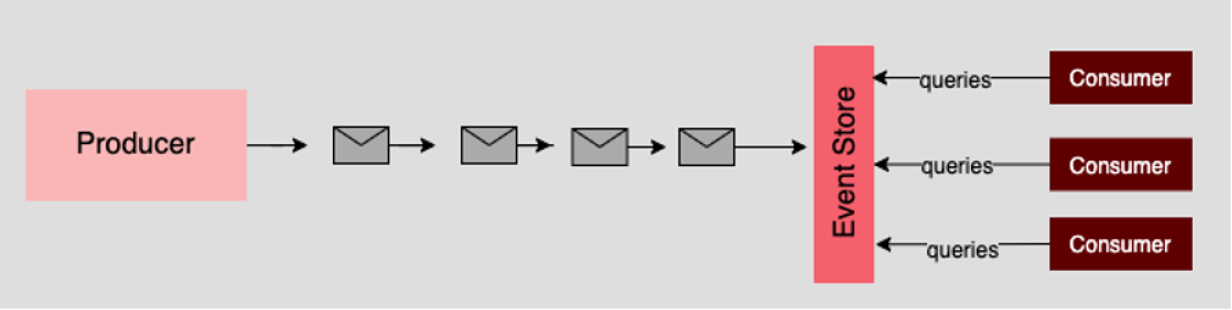
\includegraphics[width=\textwidth]{applied-thesis-chapters/chapter-2/Mẫu kiến trúc nguồn sự kiện.png}
        \caption{Mẫu kiến trúc nguồn sự kiện ~\cite{chap2bib29}}
    \end{figure}
    \item Nguồn sự kiện sẽ trả về các sự kiện theo thời gian xuất hiện (ở dạng stream). Những nơi cần sử dụng có thể đăng ký với nguồn sự kiện, sau đó sẽ được thông báo và có thể xử lý chúng nếu cần.
    \item Kiến trúc nguồn sự kiện đảm nhiệm công việc tạo ra và gửi đi các luồng tin nhắn liên tục đến một nơi lưu trữ. Mỗi tin nhắn mô tả một sự kiện trong hệ thống. Sau đó, các dịch vụ và ứng dụng khác sẽ truy vấn để tìm các sự kiện theo nhu cầu.
\end{itemize}

\paragraph{Ưu điểm}

\begin{itemize}
    \item Cực kỳ linh hoạt. Bất kỳ loại tin nhắn đều có thể được lưu trữ và truy xuất.
    \item Thích hợp cho tác vụ báo cáo dữ liệu theo thời gian thực.
    \item Các sự kiện là bất biến và chỉ có thể được thêm vào hệ thống lưu trữ. Các nơi cần sử dụng như giao diện người dùng hoặc tác vụ khởi tạo sự kiện có thể tiếp tục công viêc. Và các tác vụ xử lý sự kiện có thể chạy ở môi trường nền.
    \item Sự kiện chỉ là các đối tượng đơn giản mô tả một số hành động đã xảy ra, cùng với những dữ liệu liên quan. Chúng chỉ được ghi lại để xử lý vào thời điểm thích hợp khác. Sử dụng các sự kiện có thể đơn giản hóa việc triển khai và quản lý.
    \item Việc chỉ cho phép lưu trữ thêm các sự kiện mới cung cấp một lộ trình theo thời gian có thể được sử dụng để giám sát các hành động được thực hiện trong hệ thống. Danh sách các sự kiện cũng có thể được sử dụng để phân tích hiệu suất của ứng dụng.
\end{itemize}

\paragraph{Nhược điểm}

\begin{itemize}
    \item Các sự kiện khác nhau sẽ chứa các thông tin, định dạng khác nhau. Cần phải có một nguồn sự thật duy nhất để xác định và xác định định dạng thông báo cho một sự kiện cụ thể.
    \item Việc triển khai giải pháp nguồn sự kiện có thể đòi hỏi kiến thức chuyên môn và kỹ năng phát triển phần mềm cao.
\end{itemize}
